\clearpage
\subsection{MSVC: x86 + \olly}

Попробуем в \olly немного хакнуть программу и сделать вид, что \scanf срабатывает всегда без ошибок.
Когда в \scanf передается адрес локальной переменной, изначально в этой переменной
находится некий мусор. В данном случае это \TT{0x6E494714}:

\begin{figure}[H]
\centering
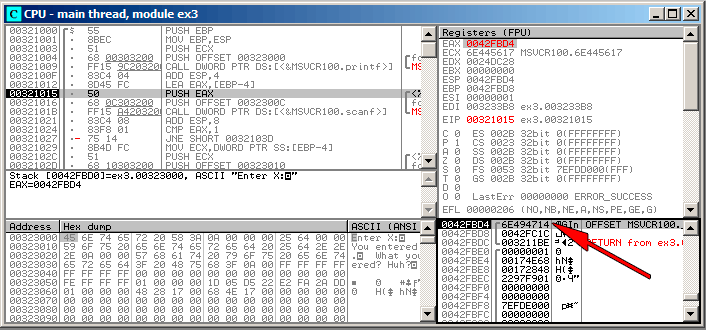
\includegraphics[scale=\FigScale]{patterns/04_scanf/3_checking_retval/olly_1.png}
\caption{\olly: передача адреса переменной в \scanf}
\label{fig:scanf_ex3_olly_1}
\end{figure}

\clearpage
Когда \scanf запускается, вводим в консоли что-то непохожее на число, например \q{asdasd}.
\scanf заканчивается с 0 в \EAX, что означает, что произошла ошибка:

\begin{figure}[H]
\centering
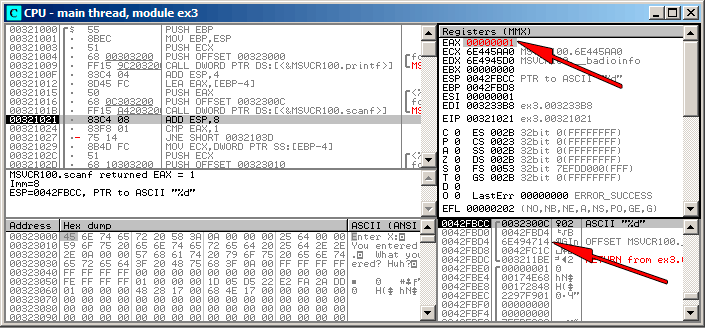
\includegraphics[scale=\FigScale]{patterns/04_scanf/3_checking_retval/olly_2.png}
\caption{\olly: \scanf закончился с ошибкой}
\label{fig:scanf_ex3_olly_2}
\end{figure}

Вместе с этим мы можем посмотреть на локальную переменную в стеке~--- она не изменилась.
Действительно, ведь что туда записала бы функция \scanf?
Она не делала ничего кроме возвращения нуля.
Попробуем ещё немного \q{хакнуть} нашу программу.
Щелкнем правой кнопкой на \EAX, там, в числе опций, будет также \q{Set to 1}.
Это нам и нужно.

В \EAX теперь 1, последующая проверка пройдет как надо, и \printf выведет значение переменной из стека.

Запускаем (F9) и видим в консоли следующее:

\begin{figure}[H]
\centering
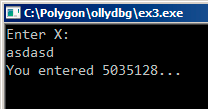
\includegraphics[scale=\FigScale]{patterns/04_scanf/3_checking_retval/olly_3.png}
\caption{консоль}
\end{figure}

Действительно, 1850296084 это десятичное представление числа в стеке (\TT{0x6E494714})!
